\usepackage{shared/cs45}
\usepackage{tikz}
\usepackage{multicol}
\usetikzlibrary{graphs}
\tikzset{>=latex}

\title{CS 45, Lecture 9}
\subtitle{Version Control}
\date{Winter 2023}
\author{Akshay Srivatsan, Ayelet Drazen, Jonathan Kula}

\newcommand{\var}[1]{\texttt{\$#1}}
\newcommand{\cmd}[1]{\mintinline{shell}{#1}}

\begin{document}

\maketitle

\frame{\titlepage}

\begin{frame}
  \frametitle{Outline}
  \tableofcontents[hidesubsections]
\end{frame}

\section{Review}

\begin{frame}{Overview}
  Last lecture, we saw:
  \begin{itemize}
    \item How to keep track of linear (ordered) histories of files
    \item How to turn non-linear version history into pseudo-linear history
  \end{itemize}
  \pause

  In this lecture, we will see:
  \begin{itemize}
    \item How to resolve merge (or rebase) conflicts
    \item How to collaborate on files with others over the internet
    \item How to back up your files and their history on the internet
  \end{itemize}
\end{frame}

\begin{frame}{Git is Confusing}
  \begin{itemize}
    \item Git is confusing!\pause
    \item Ask as many questions as you need, and don't let me move on if you
      don't yet understand something.\pause
  \end{itemize}
  \begin{center}
    \includegraphics[width=0.8\textwidth]{images/confusing.png}
  \end{center}
\end{frame}

\begin{frame}{Terminology}
  \begin{description}
    \item[\texttt{HEAD}] is the branch you're currently looking at
    \item[a branch] is a named version of a repository
    \item[fast-forwarding] means moving an old branch \enquote{forward} to add
      new commits from a more recent branch
    \item[merging] is a way of combining branches by creating a single
      \enquote{merge commit}
    \item[cherry-picking] is a way of moving commits from one branch to another
    \item[rebasing] is a way of moving an \textit{entire branch} to have a
      different \enquote{base}
  \end{description}
\end{frame}

\begin{frame}[fragile]{Rebasing}
  When you rebase a branch onto a new \enquote{base commit}:
  \mode<presentation>{\vfill}
  \begin{center}
    \begin{tikzpicture}[node distance = {15mm}, commit/.style = {draw, circle}]
      \node[commit] (A) {A};
      \node[commit] (B) [right of=A] {B};
      \only<1> {
        \alert{\node[commit, label=above:{\texttt{main}}] (C) [right of=B] {C};}
      }
      \only<2> {
        \alert{\node[commit, label=above:{\texttt{main}},
          label=below:{\texttt{feature}}] (C) [right of=B] {C};}
      }
      \only<3> {
        \node[commit, label=above:{\texttt{main}}] (C) [right of=B] {C};
      }
      \only<4-> {
        \node[commit] (C) [right of=B] {C};
      }
      \draw[->] (A) to (B);
      \draw[->] (B) to (C);
      \pause
      \pause
      \only<9-> {
        \setbeamercovered{transparent}
      }
      \uncover<-8> {
        \node[commit] (X) [below right of=C] {X};
        \draw[->] (C) to (X);
        \only<-7> {
            \alert<3-4>{\node[commit, label=below:{\texttt{feature}}] (Y) [right of=X] {Y};}
        }
        \only<8-> {
          \node[commit] (Y) [right of=X] {Y};
        }
        \draw[->] (X) to (Y);
      }
      \setbeamercovered{invisible}
      \pause
      \node[commit] (D) [right of=C] {D};
      \draw[->] (C) to (D);
      \only<-9> {
        \alert<5>{\node[commit, label=above:{\texttt{main}}] (E) [right of=D] {E};}
      }
      \only<10-> {
        \alert<5>{\node[commit] (E) [right of=D] {E};}
      }
      \draw[->] (D) to (E);
      \pause
      \pause
      \only<-9> {
        \alert<6>{\node[commit] (X2) [below right of=E] {X'};}
      }
      \only<10-> {
        \alert<6>{\node[commit] (X2) [right of=E] {X'};}
      }
      \draw[->] (E) to (X2);
      \pause
      \only<-7> {
        \alert{\node[commit] (Y2) [right of=X2] {Y'};}
      }
      \only<8-9> {
        \alert{\node[commit,label=below:\texttt{feature}] (Y2) [right of=X2] {Y'};}
      }
      \only<10-> {
        \alert{\node[commit,label=below:\texttt{feature},label=above:\texttt{main}]
          (Y2) [right of=X2] {Y'};}
      }
      \draw[->] (X2) to (Y2);
      \pause
      \pause
      \pause
    \end{tikzpicture}
  \end{center}
\end{frame}

\section{Merge Conflicts}

\begin{frame}{Merge Conflicts}
  \begin{definition}[merge conflict]
    A merge conflict is what happens when you try to combine two contradictory
    branches.  Git can't always figure out how to resolve the contradiction, so
    it'll ask the user (you).
  \end{definition}
  \pause
  \begin{itemize}
    \item Git normally resolves merge conflicts automatically.
      \pause
    \item Some conflicts have multiple valid resolutions (e.g., what if one person edited a file that another person deleted?).
      \pause
    \item If Git doesn't know what to do, it'll ask you to resolve the
      conflict. \pause
  \end{itemize}
\end{frame}

\begin{frame}[fragile]{Merge Conflicts}
  Git will tell you which files conflicted, and tell you to resolve the commits
  and commit the results:
  \begin{minted}{text}
Auto-merging hello.txt
CONFLICT (content): Merge conflict in hello.txt
Automatic merge failed; fix conflicts and then commit the result.
  \end{minted}

\end{frame}

\begin{frame}[fragile]{Merge Conflicts}{Conflict Markers}
  Git will also add conflict markers to the files:
  \begin{minted}[breaklines]{text}
Hello, my name is Akshay Srivatsan.
<<<<<<< HEAD
I'm doing my PhD in the Stanford CS department.
=======
I am a PhD student studying CS at Stanford.
>>>>>>> add-major
I'm currently co-teaching CS45 and doing research.
  \end{minted}
  This might look scary, but it's not that bad!
\end{frame}

\begin{frame}[fragile]{Merge Conflicts}{Conflict Markers: The Base Branch}
  The top part (labeled \cmd{HEAD}) are the changes in the base branch (the
  branch you're currently on):
  \begin{minted}[breaklines,escapeinside=||]{text}
Hello, my name is Akshay Srivatsan.
<<<<<<< HEAD
|\color{blue}I'm doing my PhD in the Stanford CS department.|
=======
I am a PhD student studying CS at Stanford.
>>>>>>> add-major
I'm currently co-teaching CS45 and doing research.
  \end{minted}
\end{frame}

\begin{frame}[fragile]{Merge Conflicts}{Conflict Markers: The Incoming Branch}
  The top part (labeled with a branch name or commit message) are the changes
  in the incoming branch (the one you're merging):
  \begin{minted}[breaklines,escapeinside=||]{text}
Hello, my name is Akshay Srivatsan.
<<<<<<< HEAD
I'm doing my PhD in the Stanford CS department.
=======
|\color{blue}I am a PhD student studying CS at Stanford.|
>>>>>>> add-major
I'm currently co-teaching CS45 and doing research.
  \end{minted}
\end{frame}

When you see these conflict markers, all you have to do is make the files look
the way you want them to look at the end.  In this case, I added the text
\enquote{I'm doing my PhD in the Stanford CS department.} on \cmd{main}, but I
added the text \enquote{I am a PhD student studying CS at Stanford.} on the
branch \cmd{add-major}.  When I tried to merge \cmd{add-major} into \cmd{main},
Git didn't know what to do, so it's asking me.  Now I can choose either of the
two sentences to keep, and delete the other (or I could keep both of them, if I wanted).

As an aside, you might see the name \cmd{HEAD} pop up in Git.  This basically
just means \enquote{what commit you're currently looking at}.

\begin{frame}[fragile]{Merge Conflicts}{Resolving a Conflict}
  Pick how you want to resolve the conflict (i.e., decide what the \enquote{correct} result of the merge is), and make the file look that way!
  \begin{minted}[breaklines,escapeinside=||]{text}
Hello, my name is Akshay Srivatsan.
|\color{blue}I'm a PhD student in the Stanford CS department.|
I'm currently co-teaching CS45 and doing research.
  \end{minted}
  In this case, I mixed together both versions.  The \enquote{correct} answer
  often depends on what exactly you're doing, which is why Git can't figure it
  out for you.
\end{frame}

\begin{frame}[fragile]{Merge Conflicts}{Commiting the Merge}
  Resolve all the conflicts in all the files however you want, then:
  \begin{enumerate}
    \item \cmd{git add} your changes to track them
    \item \cmd{git commit} the changes (with no message)
  \end{enumerate}

  Git will auto-generate a message, and open your \var{EDITOR} to have you
  confirm it:
  \begin{minted}[breaklines]{text}
Merge branch 'add-major'
  \end{minted}
  Save the file in your editor and close it (\cmd{:wq} in Vim), and Git will
  save the merge commit.  That's it\textemdash{}the merge conflict is gone!
\end{frame}

That's all you have to do---make the files look \enquote{correct}, then commit!
A merge conflict really isn't as bad as people sometimes make it sound; all it
means is that there are multiple ways to merge the two branches, and Git wants
you to pick one.

If you decide to use \cmd{rebase} instead, the process is pretty much the
same---just run \cmd{git rebase --continue} instead of \cmd{git commit} at the
end.

\begin{frame}[fragile]{Merge Conflicts}{Rebase Conflicts}
  Resolve all the conflicts in all the files however you want, then:
  \begin{enumerate}
    \item \cmd{git add} your changes to tell Git you fixed them
    \item \cmd{git rebase --continue}
  \end{enumerate}

  Since rebasing doesn't create a merge commit, you don't run \cmd{git commit};
  use \cmd{git rebase --continue} instead!

  Remember, rebasing happens \textit{backwards}; the base branch (the one onto
  which you're rebasing) becomes \texttt{HEAD}, and the \enquote{feature}
  branch becomes the incoming branch.
\end{frame}

\begin{frame}[fragile]{Resolving Merge Conflicts}
  To resolve a merge conflict:
  \begin{enumerate}
    \item Don't panic!
    \item Look at the files in conflict (run \cmd{git status} to see what's
      going on).
    \item Fix each conflict, one-by-one.
    \item When you're done, \cmd{git add} all the fixed files and \cmd{git
      commit}.
  \end{enumerate}

  \pause
  Let's practice!

  Merge conflicts usually happen in shared repos, so let's \textsc{clone} one
  of my repos onto your computer:

  \begin{minted}[fontsize=\small]{shell}
  git clone https://github.com/Akshay-Srivatsan/cs45-23win-demo-repo.git
  \end{minted}
\end{frame}

We'll go into more detail about how shared repositories work in the last
section of this lecture, but for now:
\begin{itemize}
  \item You can \enquote{clone} a shared repository using \cmd{git clone},
    which makes a local copy.
  \item You can \enquote{fetch} commits from the shared repository into yours
    using \cmd{git fetch}.  The commits will go into a separate branch so they
    don't conflict with yours; by convention, the branch names have the prefix
    \enquote{origin/} prepended to them, so \cmd{main} goes into
    \cmd{origin/main}.
\end{itemize}

\begin{frame}{Pulling Changes}
  You might have seen references to the \cmd{git pull} command before.  This is a combination of two commands, but the exact two depends on your Git version and configuration:
   
  \begin{description}
    \item[\cmd{git pull --ff-only}:] \cmd{git fetch} and \cmd{git merge --ff-only} (Default)
    \item[\cmd{git pull --no-rebase}:] \cmd{git fetch} and \cmd{git merge} (Old Default)
    \item[\cmd{git pull --rebase}] \cmd{git fetch} and \cmd{git rebase}
  \end{description}

  Depending on your preferences, you can configure \cmd{git pull} to do any of
  these.
\end{frame}

I personally use \cmd{git pull --rebase} the most often, since I don't like
having merge commits in my repo history.

\section{Commit Etiquette}
\begin{frame}[fragile]{Commit Messages}
  Git only saves work that we've committed, so we want to commit as often as
  possible, but\textellipsis\pause

  \begin{itemize}
    \item Other people will also look at your commit history to see what you
      did. \pause

    \item Your commit messages in the history should be short and specific, but
      descriptive enough that someone new can understand what they do. \pause

    \item Similarly, each of your commits should do a single thing, so a single
      message can describe it easily. \pause

    \item Good commits are \textsc{bisectable}; you should be able to checkout
      any commit in \cmd{main} and get a valid (e.g., compilable) state of your
      repo. \pause
  \end{itemize}

  Writing good commit messages is part of being a good programmer!
\end{frame}

These goals might seem contradictory; how do we commit as-often-as-possible,
but still make sure each of our commits are meaningful and discrete?  The
answer is: we don't!  While we're developing, we commit as often as we want.
Then, when we're ready to share our work with others, we \textit{edit our
commit history} to make it look like we made nice, easy-to-understand, discrete
commits.

\begin{frame}{Squashing Commits}
  We can commit often locally but still have meaningful commits in the end by
  \textsc{squashing} commits together with \textsc{interactive rebase}.
  \pause

  \begin{alertblock}{Editing History}
    Interactive rebasing edits history!  Don't do this on a branch you share
    with other people (like \cmd{main}).  In general, only do this on commits
    you \textbf{have not} pushed.  Otherwise, you'll have to
    \textsc{force-push} (\cmd{git push --force}) your changes, which will
    \textbf{destroy} everyone else's changes.
  \end{alertblock}
  \pause

  You can start an interactive rebase using the command \cmd{git rebase
  --interactive <base>}; for example, \cmd{git rebase --interactive main} will
  let you edit every commit that's in your branch but not in \cmd{main}.
\end{frame}

\begin{frame}[fragile]{Interactive Rebasing}
  Git will open \var{EDITOR} with a list of actions (which you can edit!).
  \begin{minted}{text}
  pick 0cd3296 start working on new file
  pick 594a80c continue working
  pick 162392b almost done
  pick bf45520 done
  pick c545ae9 oops, had a bug
  pick 9b3d056 fix the bug for real this time
  \end{minted}
  Each line represents one commit.  The first word is a \enquote{command};
  \cmd{pick} cherry-picks (i.e., includes) the commit in the new history,
  \cmd{reword} lets you edit the commit message, \cmd{edit} lets you change the
  commit contents, \cmd{squash} and \cmd{fixup} both squash the commit into the
  previous one, and \cmd{drop} removes the commit.
\end{frame}

You might notice that the default behavior here is to cherry-pick every commit.
This is the exact same as a normal (non-interactive) rebase!  What we called
\enquote{rebasing} earlier is actually a special case of editing history, but
you can go far beyond that with interactive rebasing.

\begin{frame}[fragile]{Squash and Fixup Commits}
  \vspace{-0.5em}
  Squash commits let you specify that two commits are closely related, so they
  should be combined into a single commit with both messages.

  Fixup commits let you specify that a particular commit just \enquote{fixes} a
  previous one, and therefore should be absorbed into the previous commit.
  \begin{minted}[escapeinside=||]{text}
  |\color{red}reword| 0cd3296 start working on new file
  |\color{blue}squash| 594a80c continue working
  |\color{blue}squash| 162392b almost done
  |\color{blue}squash| bf45520 done
  |\color{blue}squash| c545ae9 oops, had a bug
  |\color{blue}squash| 9b3d056 fix the bug for real this time
  \end{minted}
  \vspace{-2.5em}
\end{frame}

Note that we could also use \cmd{fixup} here, the only difference is whether
the original message gets saved or thrown away.  In this case, we're using
\cmd{reword} on the first commit anyway, so it's a moot point.

\begin{frame}[fragile]{Rewording Commits}
  When you want to \cmd{reword} a commit, Git will open \var{EDITOR} and ask
  you for a new commit message.  Enter the message you want, save, and quit.

  \begin{minted}{text}
  Add a file providing more information about the project

  # Please enter the commit message for your changes. Lines starting
  # with '#' will be ignored, and an empty message aborts the commit.
  #
  # Date:      Fri Feb 3 22:34:02 2023 -0800
  \end{minted}
\end{frame}

\begin{frame}[fragile]{Amending Commits}
  If you want to edit the most recent commit you made (i.e., \texttt{HEAD}),
  you can skip the rebase and just \textsc{amend} it, using \cmd{git commit
  --amend}.

  This will also let you edit the commit message of the last commit.
  \pause

  If you want to add to an earlier commit but don't want to do the full
  interactive rebase yet, you can use \cmd{git commit --fixup <hash>} to mark a
  commit as being a fixup commit of an earlier commit.

  You can then use \cmd{git rebase --interactive --autosquash <base>} to
  automatically absorb your fixup commits into the original commits.
  \pause

  Again, only do this if \textbf{no one else} is using your branch.
\end{frame}

\begin{frame}[fragile]{Good Commit Messages}
  \vspace{-0.5em}
  \mode<article> {
    From \href{https://github.com/stanford-stagecast/proleptic}{Stanford Stagecast: Proleptic}:
  }
  \begin{minted}[breaklines,escapeinside=||]{text}
|\color{orange}b68f706| Add training trick for handling missing notes
|\color{orange}7c0afae| Fix audio issue in metronome
|\color{orange}fa18a3d| Add a metronome for beat tracking
|\color{orange}739aa0a| Add test for per-millisecond prediction on MIDI files
|\color{orange}dc4693a| Use last eight piano roll columns to predict next
|\color{orange}eb327b4| Fix timing bug in MIDI file parser
|\color{orange}b46c6f6| Add MIDI training demo program
|\color{orange}a624b32| Switch to cross-entropy loss for MIDI classifier
|\color{orange}db3c6f3| Fix bug in MIDI parser
|\color{orange}5b0f299| Return effective learning rate from training wrapper
|\color{orange}726886d| Print more relevant training info from full-piano predictor
  \end{minted}
\end{frame}

These commit messages aren't perfect, but they're short, descriptive, and make
it clear what one thing each commit does.  They generally follow the format
\textsc{verb}-\textsc{object} (although the implied subject isn't always
consistent), and they describe which part of the codebase they're touching.

These commits are also bisectable; that means, if I notice a bug, I can
\textit{binary search} to figure out which commit introduced the bug. Git
actually has a tool for this built-in, called \cmd{git bisect}---you give it a
start and end commit (the start commit definitely doesn't have the bug, and the
end commit definitely does), and it'll checkout commits in between to help you
figure out where the bug was introduced.

\begin{frame}[fragile]{Bad Commit Messages}
  \vspace{-0.5em}
  \mode<article> {
    From \href{https://github.com/dddrrreee/cs140e-23win}{CS 140E, Winter 2023}:
  }
  \begin{multicols}{3}[]
    \begin{minted}[breaklines,escapeinside=||]{text}
|\color{orange}a527839| minor
|\color{orange}adaf72e| minor
|\color{orange}c9c6193| minor
|\color{orange}d64a6ef| minor
|\color{orange}ff2636e| minor
|\color{orange}4a988f2| minor
|\color{orange}cb901d5| minor
|\color{orange}8d4e80a| minor
|\color{orange}53b5e84| minor
|\color{orange}0321f79| minor
|\color{orange}4126899| minor
|\color{orange}f1d7231| minor
|\color{orange}cefba82| minor
    \end{minted}
    \vfill
    \pause
    \begin{minted}[breaklines,escapeinside=||]{text}
|\color{orange}44e7773| minor
|\color{orange}571c20b| minor
|\color{orange}059cb3f| minor
|\color{orange}eaa75ae| minor
|\color{orange}ebbe9db| minor
|\color{orange}13570e0| minor
|\color{orange}3e51470| minor
|\color{orange}95a0fad| minor
|\color{orange}5d2c780| minor
|\color{orange}d5caf55| minor
|\color{orange}c26b868| minor
|\color{orange}080ddf2| minor
|\color{orange}f492a3f| minor
    \end{minted}
    \vfill
    \pause
    \begin{minted}[breaklines,escapeinside=||]{text}
|\color{orange}2e67fd8| minor
|\color{orange}e530f6e| minor
|\color{orange}70387f2| minor
|\color{orange}e3d971e| minor
|\color{orange}91b236e| minor
|\color{orange}de176a8| minor
|\color{orange}461e76a| minor
|\color{orange}48cd0ff| minor
|\color{orange}0543316| minor
|\color{orange}40b48f6| minor
|\color{orange}fb0ec84| minor
|\color{orange}3a124af| added basic files.
    \end{minted}
  \end{multicols}
\end{frame}

These commit messages are useless; if you try to look back at your commit
history, you're going to have no idea what's going on.  If one of these commits
had a bug, it's hopeless to try and figure out which one introduced it.
Additionally, messages like this are often a symptom of poorly-separated
commits; it's impossible to describe what a commit does because each commit
does way too many things (or, alternatively, a single discrete change is
scattered across many commits, so there's no meaningful description of what a
single commit did).

For the record, these are both real sequences of commit messages from projects
I've worked on.  You'll probably run into both ends of this as you work with
different groups of people, but whenever you can, try to make your commit
messages more like the first example.

\section{GitHub}
\begin{frame}{GitHub}
  \begin{itemize}
    \item One of the most common reasons to use Git is to be able to
      collaborate.\pause
    \item Git has built-in support for \textsc{remote} repos, which exist on
      the internet somewhere.\pause
    \item You \textsc{clone} a remote repo to get a local copy.  You can then
      make commits on the local repo.  The remote repo is conventionally named
      \cmd{origin}.\pause
    \item You \textsc{fetch} while inside a clone, which copies the remote
      \cmd{main} branch into a branch called \cmd{origin/main}.\pause
    \item You \textsc{merge} or \textsc{rebase} your local \cmd{main} into/onto
      \cmd{origin/main}.\pause
    \item You \textsc{push} your new \cmd{main} back to the remote,
      which updates its \cmd{main} and your \cmd{origin/main}.
  \end{itemize}
\end{frame}

Remember, you can combine \cmd{fetch} and \cmd{merge} (or \cmd{rebase}) using
\cmd{pull}, if you want to.

You can actually have multiple remote repos for a single local repo.  For
example, you might have \cmd{origin} as your copy of the repo on GitHub, and
\cmd{upstream} as someone else's copy of the same repo from which you want to
cherry-pick changes.

\begin{frame}{GitHub Demo}
  Let's create a new repository on GitHub!

  You'll need the \cmd{git} command and the
  \href{https://cli.github.com}{GitHub CLI} (\cmd{gh}).

  \begin{enumerate}
    \item Go to \url{https://github.com/new} and pick a name.
    \item Click \enquote{Create repository} to continue.
    \item Run \cmd{git clone} with the URL of your new repo.
    \item Run \cmd{gh auth login} from inside your new clone.  Tell \cmd{gh}
      that you want to use it to authenticate with \cmd{git}.
    \item Make some changes (add a file), and run \cmd{git push} to upload them!
  \end{enumerate}
\end{frame}

\begin{frame}{GitHub Demo}
  Let's start collaborating!

  \begin{enumerate}
    \item On the GitHub website for your repo, go to \enquote{Settings} and
      click on \enquote{Collaborators}.
    \item Add the person sitting next to you as a collaborator!
    \item Make a clone of their repo, make some changes, then commit and push
      them.  Use \cmd{git fetch} or \cmd{git pull} to download their changes to
      your repo.
    \item What happens if you both try to edit the same file at the same time?
    \item Can you push a new branch to your partner's repo?\footnote{Hint: you
      might have to use the \cmd{--set-upstream} flag; Git will tell you
    exactly what to do.}
  \end{enumerate}
\end{frame}

\begin{frame}{Pull Requests}
  \begin{itemize}
    \item It's dangerous to give access to the \cmd{main} branch on your repo
      to everyone; someone might start messing with it!
    \item In \enquote{Settings/Branches}, you can enable \textsc{branch
      protection} for \cmd{main}.  Specifically, you can enable
      \enquote{Require a pull request before merging}.
    \item A \textsc{pull request}\footnote{This is misleadingly named, it's
      really a \enquote{merge request}} is a way to review a change before
      merging it.  You (the repo owner/maintainer) can choose whether to
      approve or reject the request.
    \item To create a pull request: create a new branch, make your changes,
      push your new branch, then run \cmd{gh pr create}.
  \end{itemize}
\end{frame}

\begin{frame}{When to use Git}
  \begin{itemize}
    \item When you want to look at past versions of a folder.

    \item When you want to be safe from accidentally overwriting your work.

    \item When you want to collaborate with other people asynchronously (use
      GitHub!).

    \item When you want to keep a backup copy of a folder with full history
      (use GitHub!).

    \item You want to \enquote{fork} a project already using Git/GitHub and
      contribute back to it.
  \end{itemize}
\end{frame}

I personally use Git pretty much whenever I write code, and even sometimes when
I'm writing prose.  Even my lecture slides for this class are tracked in
Git\textellipsis{} and lecture 6 only happened because Git saved my slides from
accidental deletion.

I actually use Git so often that I have a bunch of aliases, both in my shell
and in Git itself, to make using it faster.  From my \cmd{.zshrc}:

\begin{minted}{shell}
alias ga="git add"
alias gc="git commit"
alias gc!="git commit --amend"
alias gcmsg="git commit --message"
alias gca="git commit --all"
alias gcam="git commit --all --message"
alias gca!="git commit --all --amend"
alias gp="git push"
alias gf="git fetch"
alias gfm="git pull --no-rebase"
alias gfr="git pull --rebase"
alias gff="git merge --ff-only"
alias gst="git status"
alias gr="git rebase"
alias gri="git rebase --interactive"
alias glog="git log"
alias gco="git checkout"
alias gb="git branch"
\end{minted}

And from my \cmd{.gitconfig}:

\begin{minted}{ini}
[alias]
  co = checkout
  c = commit
  st = status
  b = branch
  hist = log --pretty=format:"%Cred%h%x09%Cgreen%cs%x09%Creset%s%x20%Cblue[%an]%Creset"
  uncommit = reset --soft HEAD^
  amend = commit --amend
  histedit = rebase -i origin/main
  unstash = stash pop
  unadd = restore --staged
  skip = update-index --skip-worktree
  unskip = update-index --no-skip-worktree
  skipped = ! git ls-files -v | grep '^S' | cut -d' ' -f2
  list = ls-files -v
  ff = merge --ff-only
  delete-remote-branch = push origin --delete
\end{minted}

I wouldn't recommend copying all of these, since some of them are particular to
my use case, but they might give you ideas of ways you can make your own Git
usage more convenient.  A git alias can be run as a git subcommand, so I can
run \cmd{git unadd hello.txt} instead of \cmd{git restore --staged hello.txt}.

\end{document}
